\documentclass{jarticle}

\usepackage[dvipdfmx]{graphicx}
\usepackage{float}
\usepackage{url}


\title{振り子の運動}
\author{2511198 肥田幸久 \\ 共同実験者 \\ 2511234 森嶋和志}
\date{2025年5月29日作成}

\begin{document}
\maketitle



\section{実験の目的}

本実験では、棒振り子の角度のデータから、角度の時間変化の様子、振り子の周期
や摩擦の大きさ等を求め、運動を解析する。



\section{実験の原理}

図\ref{fg:rod-pendulum}のような, 金属棒の端点を支点とした棒振り子を考える.

\begin{figure}[H]
  \begin{center}
    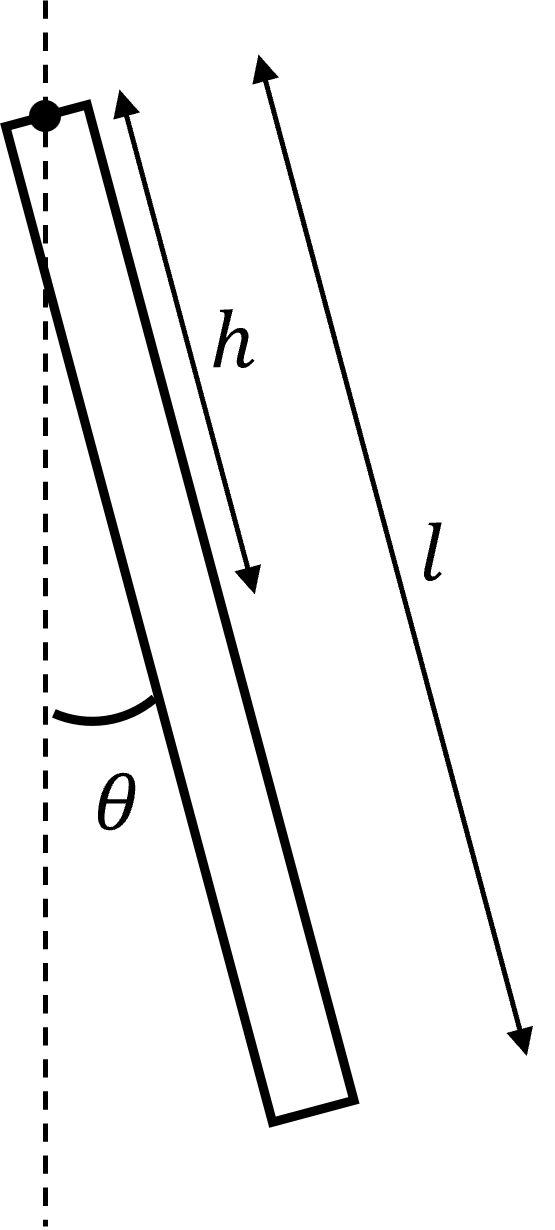
\includegraphics[width=25mm]{rod_pendulum_picture.png}
    \caption{某振り子の運動}
    \label{fg:rod-pendulum}
  \end{center}
\end{figure}

この棒振り子の長さを$l$, 重さを$m$, 振れ角を$\theta(t)$, 支点から棒の重心$(G)$までの長さを$h=l/2$とすると, 運動方程式は次式で表される.
\begin{equation}
  I\frac{d^2\theta}{dt^2}=-mghsin\theta
  \label{eq:EOM-1}
\end{equation}
ここで, $I$は棒の慣性モーメントであり, 棒の端点を回転軸とする際の$I$は,
\begin{equation}
  I=\frac{ml^2}{3}
  \label{eq:MOI}
\end{equation}
で表され, 式(\ref{eq:EOM-1})に代入すると,
\begin{equation}
  \frac{ml^2}{3}\frac{d^2\theta}{dt^2}=-mghsin\theta
  \label{eq:EOM-1.1}
\end{equation}
となる.
また, 摩擦も考慮し粘性摩擦係数を$b$とすると, 運動方程式は,
\begin{equation}
  \frac{ml^2}{3}\frac{d^2\theta}{dt^2}=-mghsin\theta-b\frac{d\theta}{dt}
  \label{eq:EOM-2}
\end{equation}
となり, 整理すると,
\begin{equation}
  \frac{d^2\theta}{dt^2}+\frac{3b}{ml^2}\frac{d\theta}{dt}+\frac{3g}{2l}sin\theta=0
  \label{eq:EOM-2.1}
\end{equation}
と表される.

また, 周期$T$は
\begin{equation}
  T=2\pi\sqrt{\frac{I}{mgh}}
  \label{eq:T-1}
\end{equation}
で表され, 整理すると
\begin{equation}
  T=2\pi\sqrt{\frac{2l}{3g}}
  \label{eq:T-2}
\end{equation}
と表される.
これより振り子の周期は長さのみに依存ことがわかる.



\section{実験方法}

本実験では図\ref{fg:rod-pendulum-method}のような装置の構成で測定を行った.
金属棒の端を角度検出センサに取り付け, 棒が振動した際の時間とともに変化する角度に対応したデータ(電圧値)をマイコンで読み取る.
マイコン内に保存されたデータをパソコンに保存し測定データとする.

\begin{figure}[H]
  \begin{center}
    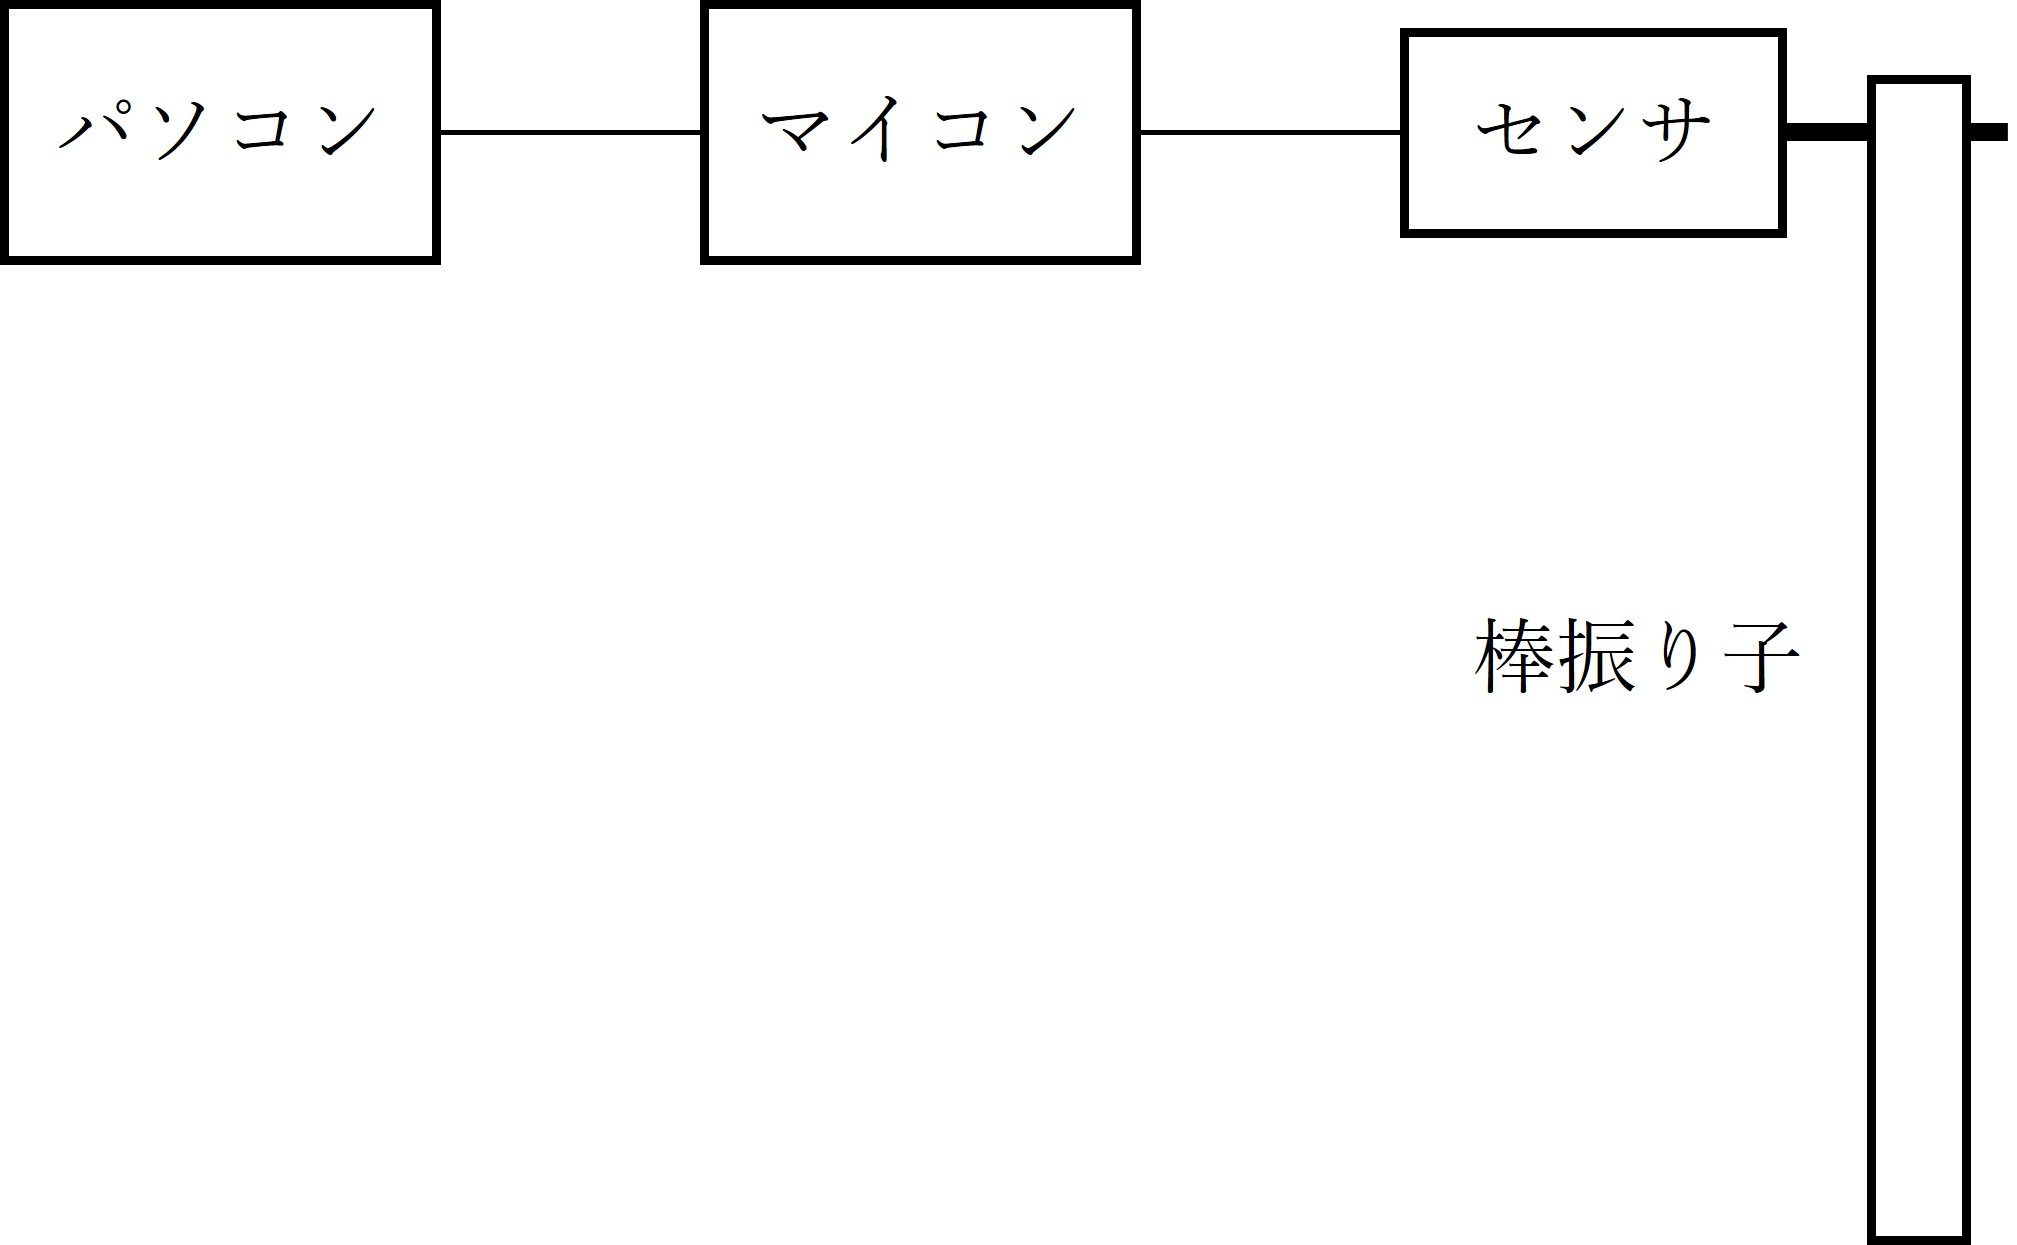
\includegraphics[width=80mm]{experimental_method_picture.jpg}
    \caption{棒振り子実験装置構成}
    \label{fg:rod-pendulum-method}
  \end{center}
\end{figure}

電圧はセンサの抵抗値が$0\Omega$のとき$0V$, $10k\Omega$のとき電源電圧である$3V$となり, それぞれ角度が$0°$と$360°$に対応している.
この電圧値は$10$bit AD変換後の値として記録されるため, マイコンに記録された角度データの値を$s$とすれば,
\begin{equation}
  \theta_{deg}=360°\times\frac{s}{2^{10}-1}
\end{equation}
により角度(degree)が求められ,
\begin{equation}
  \theta=\theta_{deg}\times\frac{\pi}{180°}
\end{equation}
により弧度法の角度(radian)を求めることができる.



\section{実験結果}


\subsection{角度の時間変化の様子}

本実験では, 長さが24cmと45cmの2種類の棒振り子を用いて測定を行った.
以下の図\ref{fg:24cm-graph}および図\ref{fg:45cm-graph}に角度の時間変化の様子をそれぞれ示す.
なお, 角度は25ms間隔で測定されている.

\begin{figure}[H]
  \begin{center}
    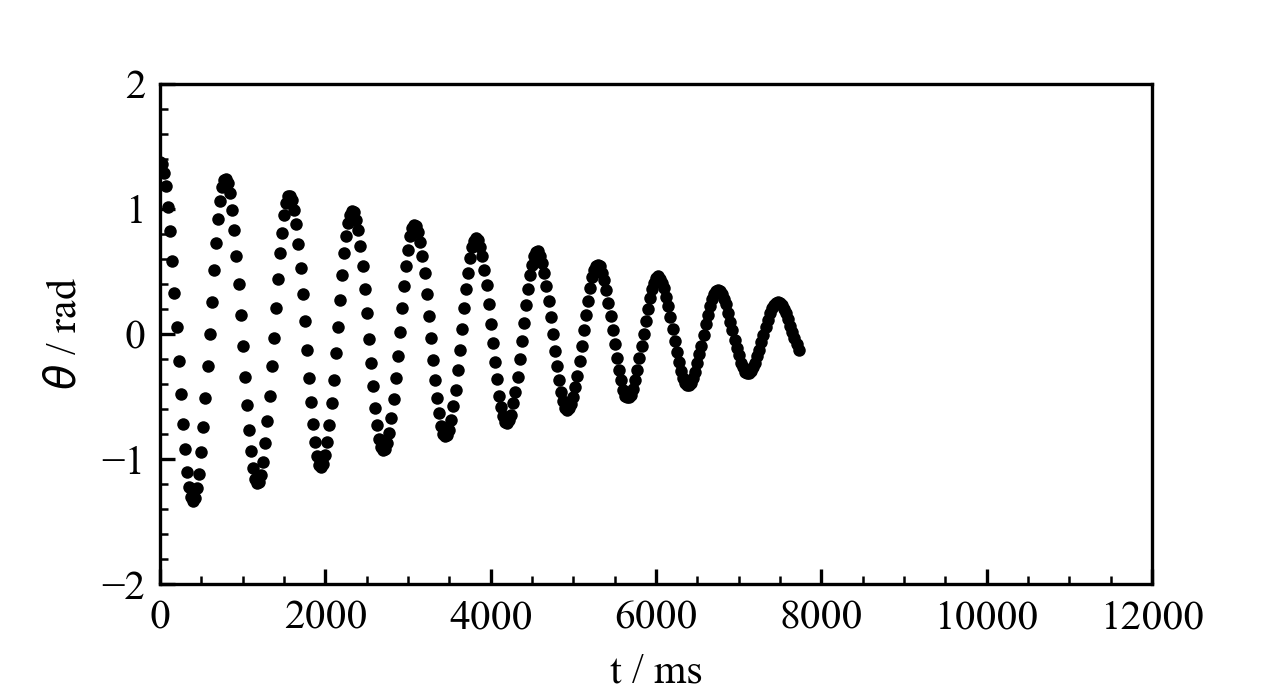
\includegraphics[width=100mm]{24cm_graph.png}
    \caption{24cmの棒振り子の角度の時間変化}
    \label{fg:24cm-graph}
  \end{center}
\end{figure}

\begin{figure}[H]
  \begin{center}
    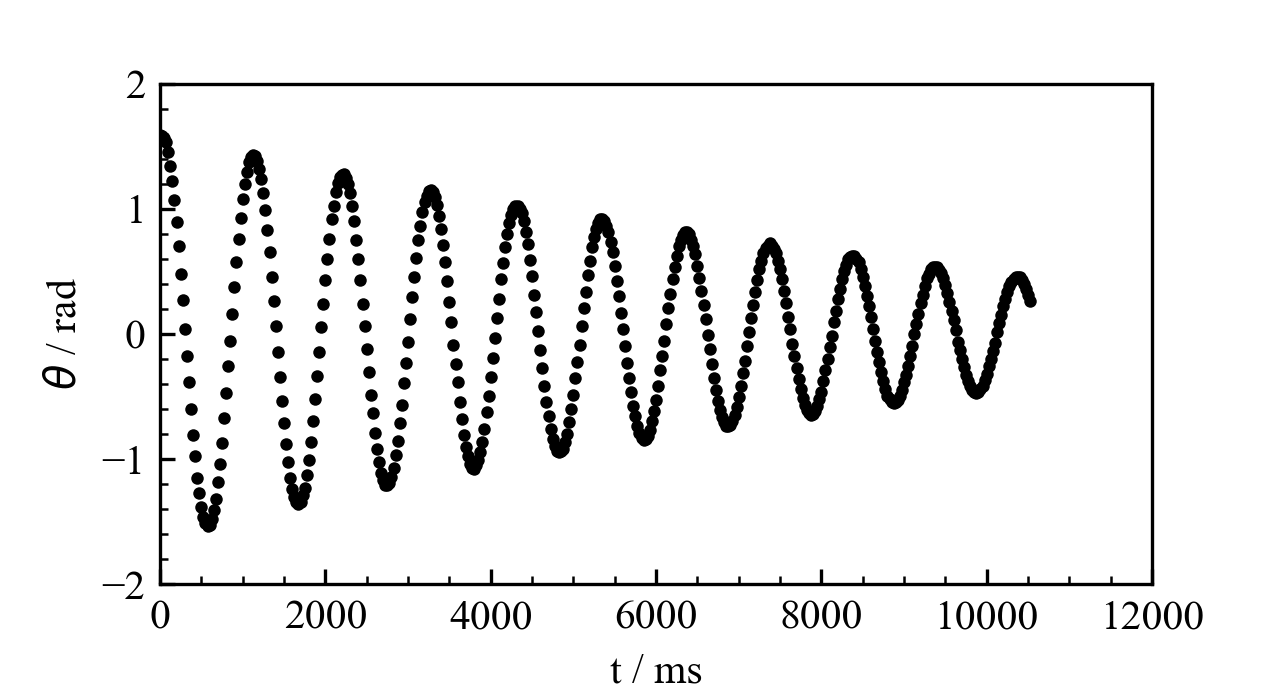
\includegraphics[width=100mm]{45cm_graph.png}
    \caption{45cmの棒振り子の角度の時間変化}
    \label{fg:45cm-graph}
  \end{center}
\end{figure}


\subsection{周期}

角度のピーク値の時間をそれぞれ抜き出し、間隔の平均を計算することで某振り子の平均の周期$\bar{T}$を求め, 式(\ref{eq:T-2})を用いた理論値$T_0$と比較し次の表\ref{tb:T}に示す.\cite{uec-atom}

\begin{table}[h]
  \centering
  \caption{棒振り子の平均の周期}
  \begin{tabular}{cccc}
    \hline
    長さ$l/\mathrm{m}$ & 平均の周期$\bar{T}/\mathrm{s}$ & 理論値$T_0/\mathrm{s}$ & 誤差$/\mathrm{s}$ \\
    \hline
    0.24 & 0.75 & 0.803 & -0.053 \\
    0.45 & 1.035 & 1.100 & -0.065 \\
    \hline
    \label{tb:T}
  \end{tabular}
\end{table}



\section{考察}

本実験で用いた金属棒の長さは, 軸から先端までの長さだが, 実際には軸を挟んだもう一方の先端までさらに$1\,\mathrm{cm}$ほどあった.
そのため, 軸から重心までの距離$h$は, 実際には$l/2$よりも軸に近い位置にあり,
\begin{equation}
  h=\frac{l+0.01}{2}-0.01
\end{equation}
と表される.

さらに, 本実験で用いたセンサの軸は一部が削れて変形していたために金属棒を軸を固定すると, 金属棒が地面に対して垂直ではなくわずかに傾いていた.
仮に地面に対して垂直な状態から$5°$傾いていたと仮定すると, 振り子の長さ$l_\perp$は,
\begin{equation}
  l_\perp=lcos5°=0.9962l
\end{equation}
となる.

これらを考慮して24cmおよび45cmの棒振り子の周期の理論値と実測値を比較すると,

\begin{table}[h]
  \centering
  \caption{棒振り子の平均の周期}
  \begin{tabular}{cccc}
    \hline
    長さ$l/\mathrm{m}$ & 実測値$T/\mathrm{s}$ & 理論値$T_0/\mathrm{s}$ & 誤差$/\mathrm{s}$ \\
    \hline
    0.24 & 0.75 & 0.796 & -0.046 \\
    0.45 & 1.035 & 1.091 & -0.056 \\
    \hline
    \label{tb:T2}
  \end{tabular}
\end{table}

となり, それぞれ1\%ほど理論値に近づく.



\begin{thebibliography}{99}
  
  \bibitem{toshidai}
  東京都市大学, ボルダの振り子による重力加速度の測定 \url{https://www.ns.tcu.ac.jp/NS/PH/homework/borda.pdf}, アクセス日:2025/5/17.

  \bibitem{uec-atom}
  小田悠介, 原子干渉計を用いた高精度な重力加速度計の開発, 電気通信大学大学院 電気通信学研究科 量子・物質工学専攻 中川研究室 \url{https://www.ils.uec.ac.jp/yellow/2005y/yellow/M-y/kodaY.pdf}, アクセス日:2025/5/25

\end{thebibliography}


\end{document}

